\documentclass{article}
\usepackage[utf8]{inputenc}
\usepackage[T1]{fontenc}
\usepackage{amsmath}
\usepackage{amsfonts}
\usepackage{amssymb}
\usepackage[dvipsnames]{xcolor}
\usepackage{enumitem}
\usepackage{titlesec}
\usepackage{graphicx}
\usepackage[total={6.5in, 9in}, heightrounded]{geometry}
\usepackage{hyperref}

\graphicspath{{graphics/}}
\setenumerate[0]{label=\alph*)}
\setlength{\parindent}{0pt}
\setlength{\parskip}{8pt}
\setlength\fboxsep{0pt}
\renewcommand{\baselinestretch}{1.6}
\titleformat{\section}
{\normalfont \Large \bfseries \centering}{}{0pt}{}

\newcommand{\s}[1]{{\color{violet} #1}}

\begin{document}

\Large Name: [YOUR NAME HERE] \hfill Homework 2 | Math 253 | Cruz Godar \vspace{4pt} \normalsize

\textit{Due Wednesday of Week 3 at the start of class}
Complete the following problems and submit them as a pdf to Canvas. 8 points are awarded for thoroughly attempting every problem, and I&#x2019;ll select three problems to grade on correctness for 4 points each. Enough work should be shown that there is no question about the mathematical process used to obtain your answers.

~\\
In problems 1--6, write the first four terms of the series and the first four partial sums.

1. $\displaystyle \sum_{m = 1}^\infty \frac{1}{m}$

2. $\displaystyle \sum_{k = 1}^\infty \frac{1}{k^2}$

3. $\displaystyle \sum_{i = 1}^\infty \frac{1}{i + 1} - \frac{1}{i}$

4. $\displaystyle \sum_{n = 1}^\infty (-1)^n$

5. $\displaystyle \sum_{n = 0}^\infty \frac{1}{10^n}$

6. $\displaystyle \sum_{n = 1}^\infty n$

~\\

7. For problems 3--6, find an explicit formula for $S_n$ the $n$ partial sum, and use it to find the value of the series. (Hint: for problem 6, try finding \textit{double} the partial sum first by adding $1 + 2 + \cdots + n$ to $n + (n - 1) + \cdots + 1$ Can you find a way to simplify those two sums when added together?)

~\\
In problems 8--13, find the value of the series.

8. $\displaystyle \sum_{m = 0}^\infty \frac{1}{3^m}$

9. $\displaystyle \sum_{k = 3}^\infty (-5)^{-k}$

10. $\displaystyle \sum_{n = -2}^\infty \left( -\frac{1}{2} \right)^n + \left( \frac{1}{4} \right)^n$

11. $\displaystyle \sum_{n = 1}^\infty \left( \cos\left( \frac{\pi}{n} \right) - \cos\left( \frac{\pi}{n + 2} \right) \right)$

12. $\displaystyle \sum_{n = 1}^\infty 3^n\frac{1 - 2n}{n(n + 1)}$

13. $\displaystyle \sum_{m = 1}^\infty \ln\left( \frac{m}{m + 1} \right)$

~\\

14. Does every telescoping series of the form $\displaystyle \sum_{n = 1}^\infty (a_{n + 1} - a_n)$ converge to $-a_1$ Why or why not?

15. If $\displaystyle \sum_{n = 1}^\infty a_n$ converges and $|b_n| < |a_n|$ for all $n$ does $\displaystyle \sum_{n = 1}^\infty b_n$ necessarily converge?

~\\
The Koch snowflake is a fractal, an object that is infinitely detailed no matter how far you zoom in. We&#x2019;ll begin with an equilateral triangle with side lengths equal to 1, and remove the middle third of each side, replacing it with two additional sides of equal length. Then repeat this for all 12 sides of the new figure, and so on. The limit of this sequence of figures is the completed Koch snowflake. A diagram of the first four steps is on the next page --- the green lines are what has been most recently removed and are not part of the snowflake.

\begin{center}
	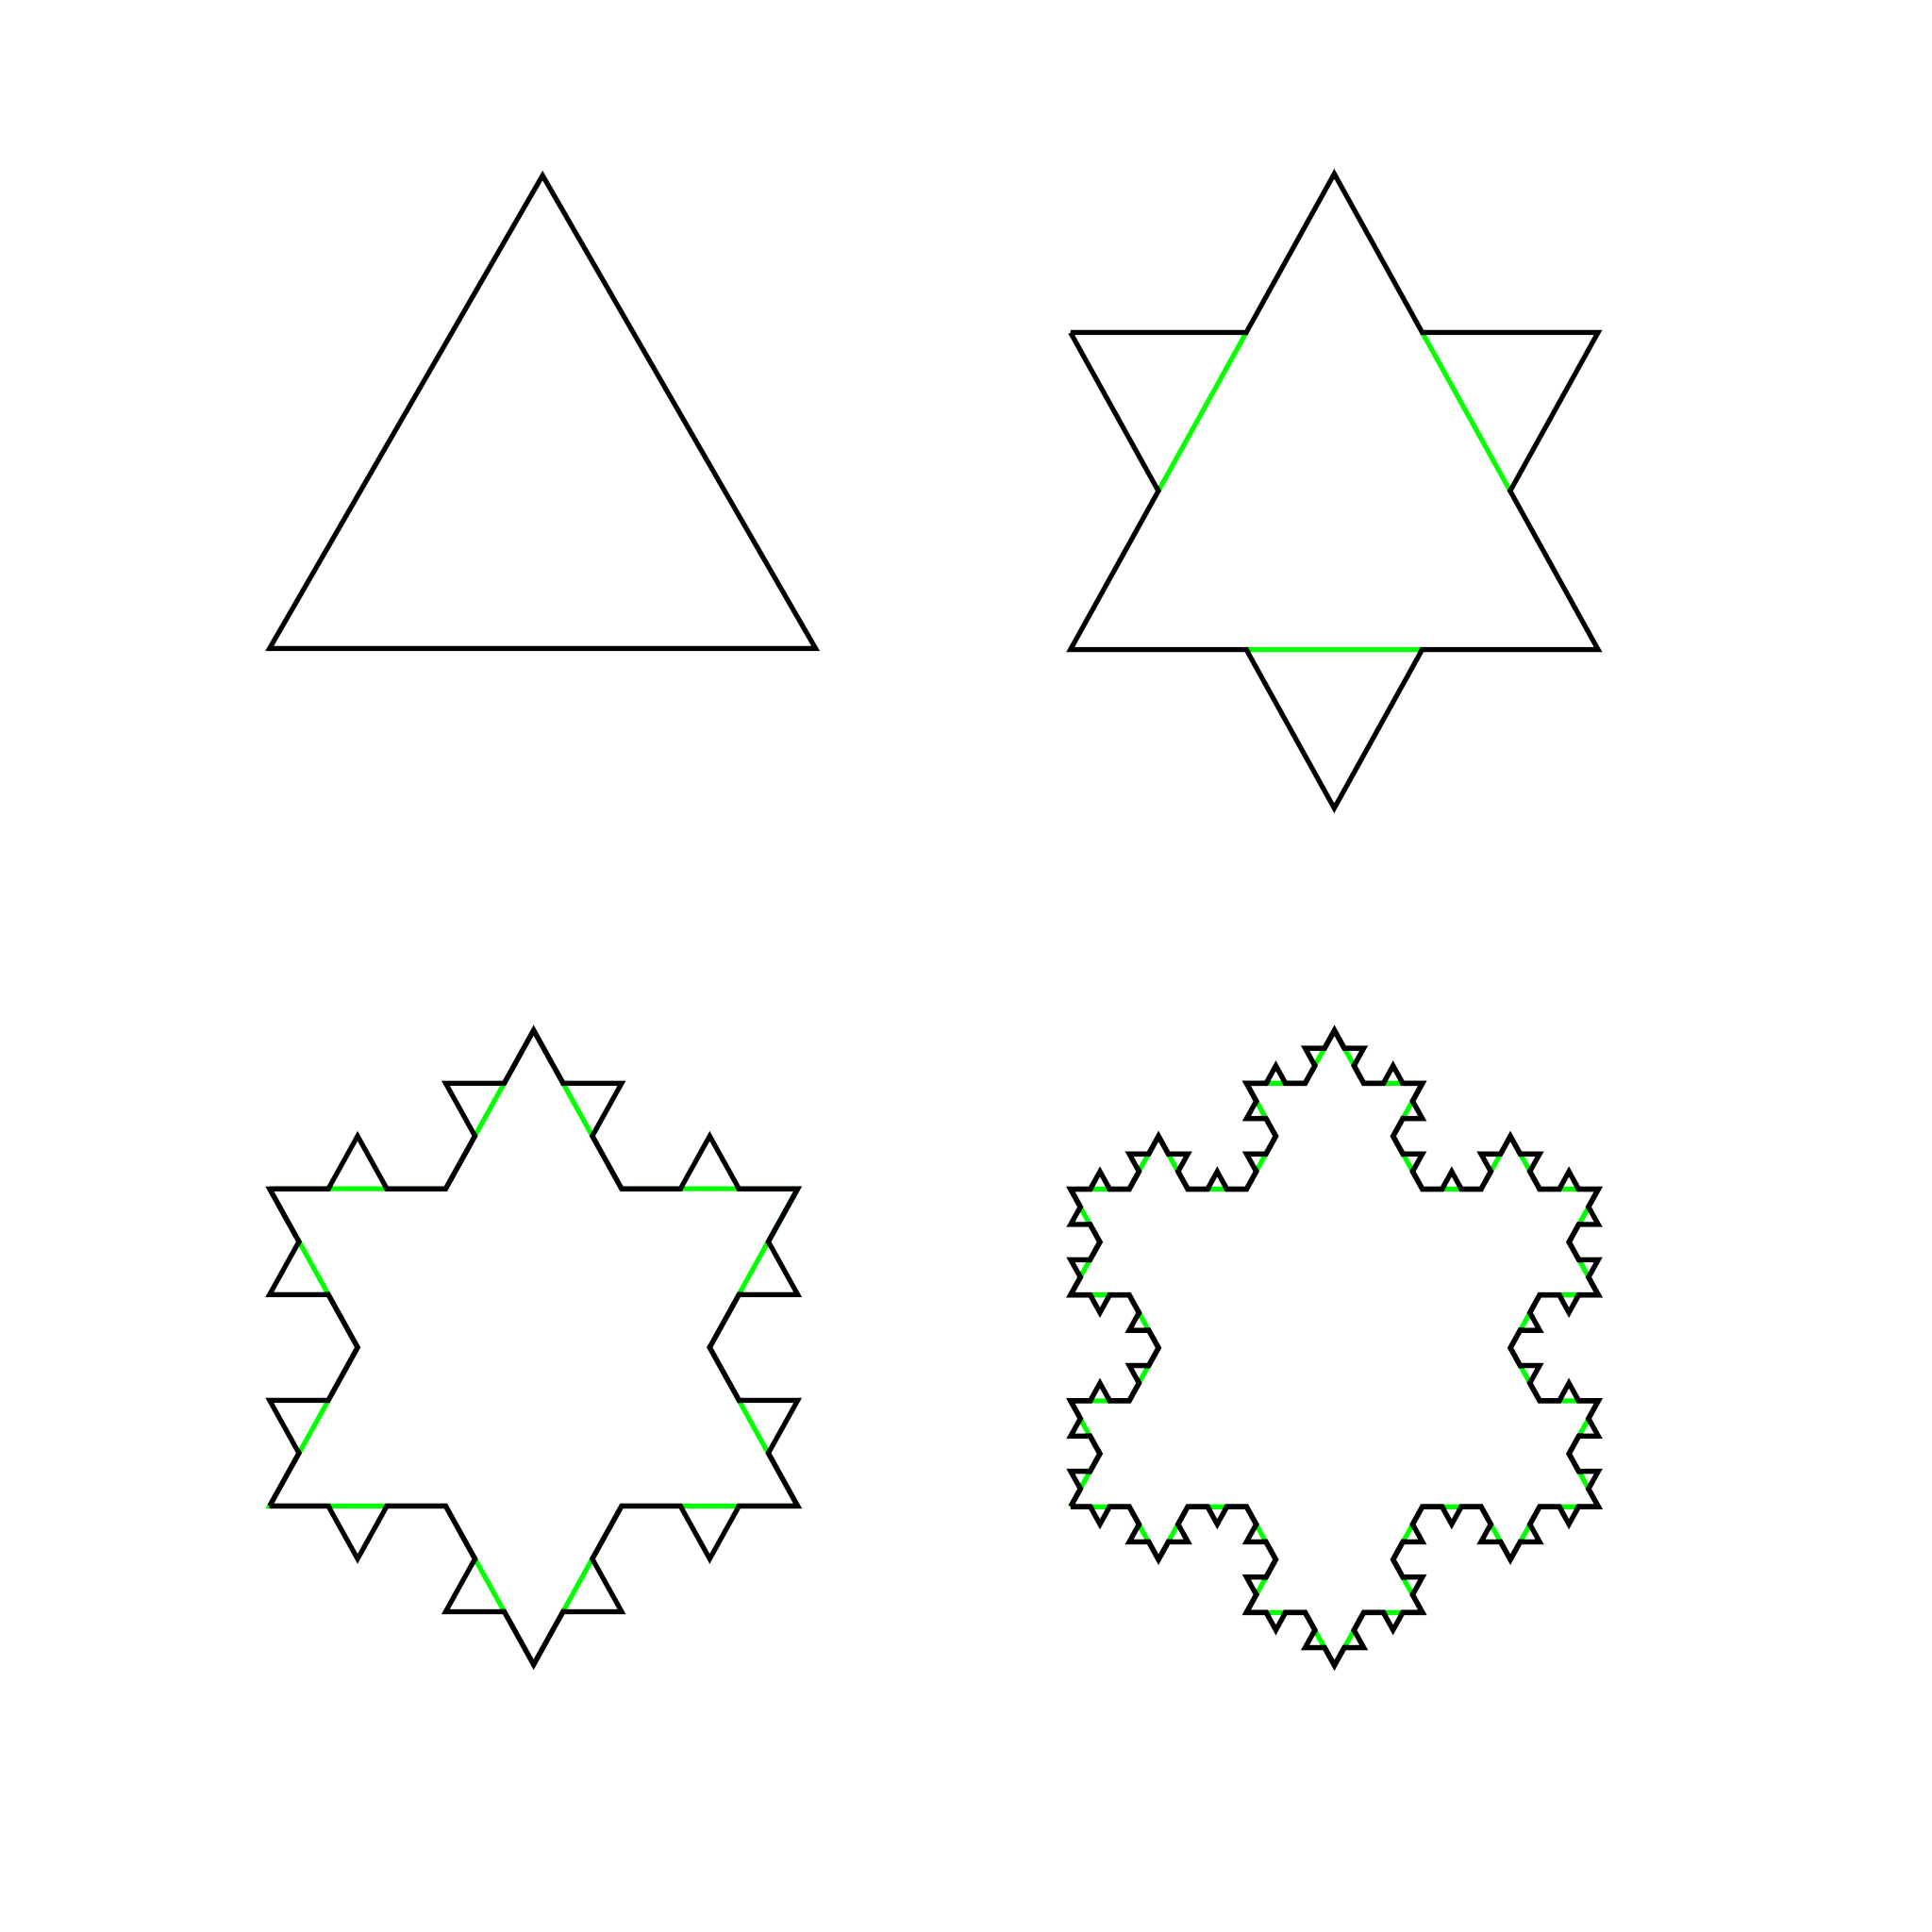
\includegraphics[width=0.5\linewidth]{koch-snowflake.png}
\end{center}

16. Let $c_n$ be the number of edges in the snowflake at step $n$ and let $l_n$ be their lengths. For example, $c_0 = 3$ since we start with a triangle, and $l_0 = 1$ since the sides of the triangle all have length $1$ In the next step, $c_1 = 12$ and $l_1 = \dfrac{1}{3}$ Find explicit formulas for $c_n$ and $l_n$

17. Let $p_n$ be the perimeter of the snowflake at step $n$ Using your answer to question 16, find an explicit formula for $p_n$ Then find the perimeter of the completed snowflake by taking the limit of the sequence $(p_n)$

18. Let $A$ be the area of the completed Koch snowflake and let $a_n$ be the amount the area increases at step $n$ where $n \geq 1$ For example, step 1 is going from the original triangle to the six-pointed star. That adds three triangles, each of area $\dfrac{\sqrt{3}}{36}$ Therefore, $a_1 = \dfrac{\sqrt{3}}{12}$ Using your answer to question 16, find an explicit formula for $a_n$ The area of the original triangle is $\dfrac{\sqrt{3}}{4}$ and so the total area $A$ of the completed snowflake is
$$$
	A = \frac{\sqrt{3}}{4} + \sum_{n = 1}^\infty a_n.
$$$
Find $A$

\end{document}